\section{Qu'est ce que le reconnaissance de formes ?}

La \textbf{Reconnaissance de forme}, ou \textit{Shape Matching} en anglais, est la discipline scientifique dont l'objet d'étude est l'ensemble des méthodes et techniques permettant d'identifier un \textbf{\textit{motif}} et d'en déterminer par la suite la catégorie. C'est un domaine très lié aux méthodes dites de \textbf{Vision par Ordinateur}, ou \textit{Computer Vision} en anglais.

Ses applications sont très larges et vont de la voiture autonome qui doit pouvoir identifier un vaste ensemble de formes variées (panneaux, signalisation au sol, véhicules, personnes, animaux, obstacles ...), au contrôle qualité partiellement ou totalement automatisé.

De manière plus large, on retrouve également ce type d'algorithme en sécurité informatique ou sécurité civile pour détecter un \textit{motif de comportement anormal} : détection d'intrusion réseau, lutte anti-terrorisme \ldots

 \begin{figure}[H]
    \centering
    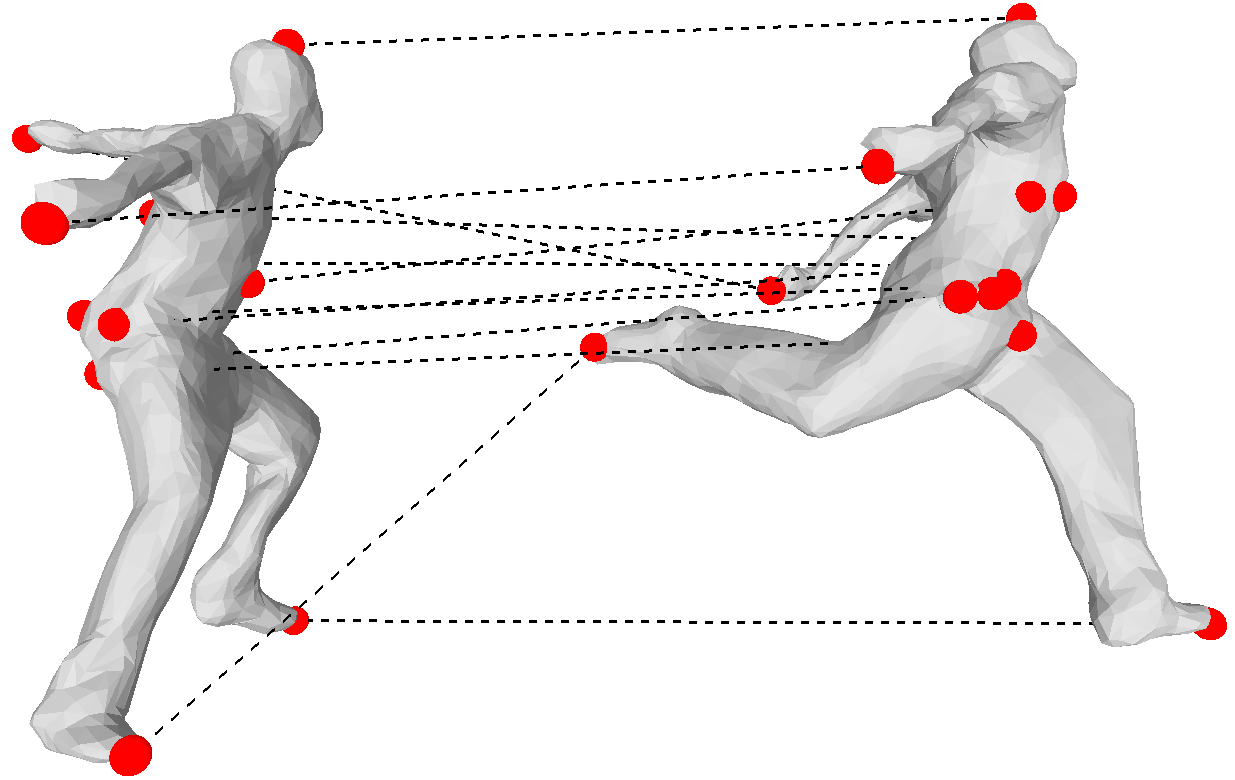
\includegraphics[height=6cm]{shapeMatching.png}
	\caption{Sortie typique d'un algorithme de reconnaissance de formes 2D/3D~\cite{shapeMatchingImg}}\label{image.shapeMatching} 
\end{figure}

 \begin{figure}[H]
    \centering
    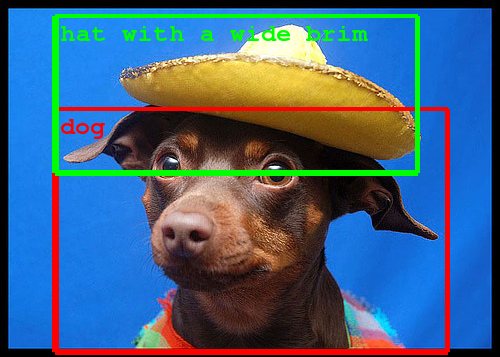
\includegraphics[height=6cm]{computerVision.png}
	\caption{Sortie typique d'un algorithme de vision par ordinateur~-~Source: \href{http://googleresearch.blogspot.fr/2014/09/building-deeper-understanding-of-images.html}{Google Research}}\label{image.computerVision} 
\end{figure}